\documentclass[11pt]{article}
\usepackage[a4paper,margin=18mm]{geometry}
\usepackage{fontspec}
\setmainfont{Latin Modern Roman}
\usepackage{amsmath,amssymb,amsthm,amscd,graphicx,color}
\usepackage{xurl}
\usepackage[unicode,hidelinks]{hyperref}
\allowdisplaybreaks
\setlength\emergencystretch{3em}
%\usepackage{epic,eepic} % for figures
\usepackage[mathscr]{eucal} %  use \EuScript (\mathcal unchanged)


\numberwithin{equation}{section}


\newtheorem{Theorem}{Theorem}[section]
\newtheorem{Proposition}[Theorem]{Proposition}
\newtheorem{Lemma}[Theorem]{Lemma}
\newtheorem{Corollary}[Theorem]{Corollary}
\theoremstyle{definition}
\newtheorem{Definition}[Theorem]{Definition}
\newtheorem{Example}[Theorem]{Example}
\newtheorem{Remark}[Theorem]{Remark}

%% Next two commands enlarge space for figures on the top of a page
\renewcommand{\textfraction}{0.05}
\renewcommand{\topfraction}{0.95}


\makeatletter\newlabel{subsec:back}{{2.3}{}{Original source locator}{}{}}\makeatother
\makeatletter\newlabel{eq:xi}{{2.27}{}{Original source locator}{}{}}\makeatother
\makeatletter\newlabel{eq:case2}{{7.1}{}{Original source locator}{}{}}\makeatother
\makeatletter\newlabel{sec:extension}{{7}{}{Original source locator}{}{}}\makeatother
\begin{document}
\begin{center}\Large For every integer n at least four, the formal sine-Gordon Y-system has half-period four n minus two exchanging its two terminal nodes and full period eight n minus four\end{center}
\noindent\textbf{Stable ID:} 2820\par
\noindent\textbf{Authors:} Tomoki Nakanishi; Roberto Tateo\par
\noindent\textbf{Original work:} Dilogarithm Identities for Sine-Gordon and Reduced Sine-Gordon Y-Systems\par
\noindent\textbf{Version:} Official SIGMA 6 (2010) article 085, DOI 10.3842/SIGMA.2010.085; journal PDF and native TeX acquired 2026-10-01, exact bytes pinned by SHA256\par
\noindent\textbf{Selected task scope:} Theorem2.3 for integer n>=\allowbreak{}4 and the exact SG formal Y-system of Definition2.1 in the semifield and multiplicative subgroup of Definition2.2. For all i in1,...,n+\allowbreak{}1 and u inZ, Y\_i(u+\allowbreak{}4n-2)=\allowbreak{}Y\_omega(i)(u), where omega fixes1,...,n-1 and exchanges n,n+\allowbreak{}1; hence Y\_i(u+\allowbreak{}8n-4)=\allowbreak{}Y\_i(u). No minimal-period assertion, analytical PDE claim, dilogarithm identity, reduced-SG or additional continued-fraction family.\par
\noindent\textbf{Difficulty:} H2: The unusual long-range first recurrence is not an ordinary Dynkin Y-system, so its period cannot be read from a single Coxeter number. The author constructs a shared-vertex mutation quiver and factors its tropical coefficients into two independently tracked families. Four time regions with type D\_n and D\_(n-1) root dynamics and explicit even/odd terminal-node formulas establish the tropical return, which the cited general lifting theorem transports to the original formal recurrence.\par
\noindent\textbf{Editorial boundary note (not author text):} The complete original Theorem2.3 half/full sine-Gordon Y-system periodicity is retained for the exact formal semifield/group recurrence and every integer n>=\allowbreak{}4. The full shared-vertex mutation quiver, parity/embedding maps, tropical coefficient factorization, four time regions of D\_n and D\_(n-1) root dynamics, explicit terminal-node formulas and complete tropical-to-formal lifting argument are bundled. Original cluster-algebra definitions are retained from AppendixA; cited general lifting and finite-type root results remain prior prerequisites. Other dilogarithm, T-system, reduced-SG and later continued-fraction results are uncounted context; no minimal-period claim is selected.\par
\noindent\textbf{Source:} \url{https://sigma-journal.com/2010/085/}\quad DOI: \url{https://doi.org/10.3842/SIGMA.2010.085}\par
\noindent\textbf{License and attribution:} Copyright retained by the named authors. Published by SIGMA under CC BY 4.0: \url{https://creativecommons.org/licenses/by/4.0/}. Source: \url{https://sigma-journal.com/about.html}. Adaptation consists of standalone excerpt formatting, cover and numbering restoration; original author language and mathematical text are retained.\par
\noindent\textbf{External original locator subsec:back:} Section2.3 gives separately unselected integrable-model background; the formal recurrence/semifield definitions and full new quiver/tropical proof are retained.\par
\noindent\textbf{External original locator eq:xi:} Equation2.27 gives the integrable-model parameter interpretation; it is not used to prove the selected formal Y-system period.\par
\noindent\textbf{External original locator eq:case2:} Equation7.1 concerns a separately unselected later continued-fraction extension; no such extension is selected.\par
\noindent\textbf{External original locator sec:extension:} Section7 concerns separately unselected further extensions.\par
\medskip\hrule\medskip\noindent\textbf{Author text begins below.}\par
\setcounter{section}{1}
\setcounter{subsection}{0}
\setcounter{subsubsection}{0}
\setcounter{Theorem}{0}
\setcounter{equation}{0}
% Original source lines 231--550
\section{Main results}
\label{sec:main}


\subsection{Results for sine-Gordon Y-systems}

\begin{figure}[t]
\centerline{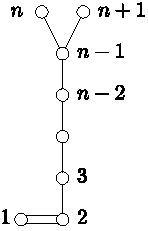
\includegraphics{../assets/2820/Nakanishi-Fig1.pdf}}
\caption{The diagram $X_n$.}
\label{fig:X}
\end{figure}

With an integer $n \geq 4$, we associate a
diagram $X_n$ in Fig.~\ref{fig:X}.
%For later use, we also attach the properties
%$\circ/\bullet$ and $+/-$ to each vertex of $X_n$.
The diagram $X_n$ should {\em not\/} be regarded as an
ordinary Dynkin diagram,
since the horizontality and verticality of
segments also carry information.
It appeared in \cite{Tateo95}
and encodes the structure of the Y-systems
which we are going to introduce now.
Let $\mathcal{I}_n=\{1,\dots,n+1\}\times \mathbb{Z}$.

\begin{Definition}
\label{def:SGY}
Fix an integer $n \geq 4$.
The sine-Gordon (SG)
Y-system $\mathbb{Y}_{n}(\mathrm{SG})$
is the following system of relations for
a family of variables
 $\{Y_i(u) \mid (i,u)\in \mathcal{I}_n \}$,
\begin{gather}
Y_1\left(u-n+1\right)
Y_1\left(u+n-1\right)
=
\left(\prod_{j=2}^{n-1}(1+Y_j(u-n+j))(1+Y_j(u+n-j))\right)\nonumber\\
\phantom{Y_1\left(u-n+1\right)
Y_1\left(u+n-1\right)
=}{}
 \times (1+Y_n(u))(1+Y_{n+1}(u)),
\nonumber\\
Y_2(u-1) Y_2(u+1)
=
\frac
{1+Y_1(u)}
{1+Y_3(u)^{-1}}
,\nonumber\\
Y_i(u-1)Y_i(u+1)
=
\frac{1}{\prod\limits_{j:j\sim i} (1+Y_j(u)^{-1})},
\qquad i=3,\dots,n+1,\label{eq:Y1}
\end{gather}
where $j\sim i$ means that $j$ is adjacent to $i$ in $X_n$.
\end{Definition}

In \cite{Tateo95}, a more general
family of Y-systems was associated with
a rational parameter $\xi$,
which is related  the coupling constant $\beta$
 of the SG model by \eqref{eq:xi}.
The system \eqref{eq:Y1} corresponds to
the special case
\begin{gather}
\label{eq:case1}
\xi=\frac{n-1}{n}=
\cfrac{1}{ 1 +
\cfrac{1}{n-1}
},
\end{gather}
namely, $F=2$, $n_1=1$, and $n_2=n$ in the notation
in \cite{Tateo95}.
The variable $u$ here is related to the variable $\theta$
in \cite{Tateo95} by $u = (2n/\pi\sqrt{-1})\theta$.
Later in Section~\ref{subsec:back} we explain more about the background
of~\eqref{eq:Y1}.

\begin{Definition}
\label{def:YC}
Let $\EuScript{Y}_{n}(\mathrm{SG})$
be the semif\/ield (Appendix \ref{sec:groc}(i)) with generators
$Y_i(u)$
 $((i,u)\in \mathcal{I}_{n})$
and relations $\mathbb{Y}_{n}(\mathrm{SG})$.
Let $\EuScript{Y}^{\circ}_{n}(\mathrm{SG})$
be the multiplicative subgroup
of $\EuScript{Y}_{n}(\mathrm{SG})$
generated by
$Y_i(u)$, $1+Y_i(u)$
 $((i,u)\in \mathcal{I}_{n})$.
(Here we use the symbol $+$ instead of $\oplus$
for simplicity.)
\end{Definition}
The f\/irst main result of the paper is
the following two theorems conjectured by
\cite{Tateo95}.

\begin{Theorem}[Periodicity]
\label{thm:Yperiod}
The following relations hold in $\EuScript{Y}^{\circ}_{n}(\mathrm{SG})$.
\begin{enumerate}\itemsep=0pt
\item[$(i)$] Half periodicity: $Y_i(u+4n-2)=Y_{\omega(i)}(u)$, where
$\omega$ is an involution of the set $\{1,\dots,n+1\}$
defined by $\omega(n)=n+1$, $\omega(n+1)=n$,
and $\omega(i)=i$ $(i=1,\dots,n-1)$.
\item[$(ii)$] Full periodicity: $Y_i(u+8n-4)=Y_i(u)$.
\end{enumerate}
\end{Theorem}

In our proof of Theorem \ref{thm:Yperiod}
we have  a natural interpretation
of the  half period
\[
4n-2=h(D_n)+2+h(D_{n-1})+2
\]
in terms of the Coxeter number  $h(D_n)=2n-2$ of type $D_n$.

Let $L(x)$ be the {\em Rogers dilogarithm function\/}
 \cite{Lewin81}
\begin{gather*}
%\label{eq:L0}
L(x)=-\frac{1}{2}\int_{0}^x
\left\{ \frac{\log(1-y)}{y}+
\frac{\log y}{1-y}
\right\} dy,
\qquad 0\leq x\leq 1.
\end{gather*}
It satisf\/ies the following relation
\begin{gather}
\label{eq:euler}
L(x)+L(1-x)=\frac{\pi^2}{6},
\qquad 0\leq x\leq 1.
\end{gather}

\begin{Theorem}[Functional dilogarithm identities]
\label{thm:dilog}
Suppose that a family of positive real numbers
$\{ Y_i(u) \mid (i,u)\in \mathcal{I}_n\}$ satisfies
$\mathbb{Y}_n(\mathrm{SG})$.
Then, we have the identities
\begin{gather}
\label{eq:DI}
\frac{6}{\pi^2}
\sum_{
\genfrac{}{}{0pt}{1}
{
(i,u)\in \mathcal{I}_{n}
}
{
0\leq u < 8n-4
}
}
L\left(
\frac{Y_i(u)}{1+Y_i(u)}
\right)
 =8(2n-1),\\
\label{eq:DI'}
\frac{6}{\pi^2}
\sum_{
\genfrac{}{}{0pt}{1}
{
(i,u)\in \mathcal{I}_{n}
}
{
0\leq u < 8n-4
}
}
L\left(
\frac{1}{1+Y_i(u)}
\right)
 =4(n-1)(2n-1).
\end{gather}
\end{Theorem}
Two identities
\eqref{eq:DI} and \eqref{eq:DI'}
are equivalent to each other due to \eqref{eq:euler}.


Using this opportunity, we introduce
another system of relations
 accompanying  $\mathbb{Y}_{n}(\mathrm{SG})$.
\begin{Definition}
Fix an integer $n \geq 4$.
The sine-Gordon (SG)
T-system $\mathbb{T}_{n}(\mathrm{SG})$
is the following system of relations for
a family of variables
 $\{T_i(u) \mid (i,u)\in \mathcal{I}_n \}$,
\begin{gather}
T_1\left(u-n+1\right)
T_1\left(u+n-1\right)
=
T_2(u)+1,\nonumber\\
T_2(u-1) T_2(u+1)
=
T_1(u-n+2)T_1(u+n-2)+T_3(u),
\nonumber\\
T_i(u-1)T_i(u+1)
=
T_1(u-n+i)T_1(u+n-i)
+ \prod_{j:j\sim i} T_j(u),
\qquad i=3,\dots,n-1,
\nonumber\\
T_{n}(u-1)T_{n}(u+1)
=
T_1(u) + T_{n-1}(u),
\nonumber\\
T_{n+1}(u-1)T_{n+1}(u+1)
=
T_1(u) + T_{n-1}(u),\label{eq:T1}
\end{gather}
where $j\sim i$ means that $j$ is adjacent to $i$ in $X_n$.
\end{Definition}

There are two connections between
$\mathbb{Y}_{n}(\mathrm{SG})$ and $\mathbb{T}_{n}(\mathrm{SG})$.
The f\/irst connection is a formal one.
Set
\begin{gather}
\label{eq:di}
d_1=n-1, \qquad d_i=1,\qquad i=2,\dots,n-1,
\end{gather}
and let us  write \eqref{eq:Y1}
in a unif\/ied manner as
\begin{gather}
\label{eq:Yuni}
Y_i\left(u-d_i\right)
Y_i\left(u+d_i\right)
=
\frac{
{\prod\limits_{(j,v)\in \mathcal{I}_{n}}
(1+Y_j(v))^{G_+(j,v;i,u)}
}
}
{\prod\limits_{(j,v)\in \mathcal{I}_{n}}
(1+Y_j(v)^{-1})^{G_-(j,v;i,u)}
}.
\end{gather}
Then, \eqref{eq:T1} is written as
\begin{gather}
\label{eq:Tuni}
T_i\left(u-d_i\right)
T_i\left(u+d_i\right)
=
\prod_{(j,v)\in \mathcal{I}_{n}}
T_j(v)^{G_+(i,u;j,v)}
+
\prod_{(j,v)\in \mathcal{I}_{n}}
T_j(v)^{G_-(i,u;j,v)}.
\end{gather}
Note that we took the `transpositions'
of $G_+$ and $G_-$ in \eqref{eq:Tuni}.
The second connection is an algebraic one.
Suppose that $\{ T_i(u) \mid (i,u)
\in \mathcal{I}_n\}$ satisf\/ies
the T-system $\mathbb{T}_n(\mathrm{SG})$.
Set
\[
Y_i(u)
=
\frac{\prod\limits_{(j,v)\in \mathcal{I}_{n}}
T_j(v)^{G_+(i,u;j,v)}
}
{\prod\limits_{(j,v)\in \mathcal{I}_{n}}
T_j(v)^{G_-(i,u;j,v)}}.
\]
Then, $\{ Y_i(u) \mid (i,u)
\in \mathcal{I}_n\}$ satisf\/ies
the Y-system $\mathbb{Y}_n(\mathrm{SG})$.
One may check the claim directly at this moment
using $\mathbb{T}_n(\mathrm{SG})$
(with some ef\/fort).
Alternatively and better, one can automatically obtain  it from
 \cite[Proposition 3.9]{Fomin07}
once we formulate these systems by a cluster algebra
in the next section.

\begin{Definition}
\label{defn:TC}
Let $\EuScript{T}_{n}(\mathrm{SG})$
be the commutative ring over $\mathbb{Z}$
with identity element,  with gene\-ra\-tors
$T_i(u)^{\pm 1}$ $((i,u)\in \mathcal{I}_{n})$
and relations $\mathbb{T}_{n}(\mathrm{SG})$
together with $T_i(u)T_i(u)^{-1}=1$.
Let $\EuScript{T}^{\circ}_{n}(\mathrm{SG})$
be the subring of $\EuScript{T}_{n}(\mathrm{SG})$
generated by
$T_i(u)$ $((i,u)\in \mathcal{I}_{n})$.
\end{Definition}

The following theorem can be proved simultaneously
with Theorem \ref{thm:Yperiod}.

\begin{Theorem}[Periodicity]
\label{thm:Tperiod}
The following relations hold in $\EuScript{T}^{\circ}_{n}(\mathrm{SG})$.
\begin{enumerate}\itemsep=0pt
\item[$(i)$] Half periodicity: $T_i(u+4n-2)=T_{\omega(i)}(u)$, where
$\omega$ is the  one in Theorem~{\rm \ref{thm:Yperiod}}.
\item[$(ii)$] Full periodicity: $T_i(u+8n-4)=T_i(u)$.
\end{enumerate}
\end{Theorem}

\begin{Remark}
Actually,
 $\mathbb{Y}_n(\mathrm{SG})$ and  $\mathbb{T}_n(\mathrm{SG})$
are also considered for $n=3$,
and they coincide with the Y and T-systems of
type $B_2$ with level $2$ in~\cite{Kuniba94a}.
Theorems~\ref{thm:Yperiod}, \ref{thm:dilog},
and~\ref{thm:Tperiod} remain valid for $n=3$
due to~\cite{Inoue10a}.
\end{Remark}

All the results in this subsection will be
extended to a more general case~\eqref{eq:case2}
later in Section~\ref{sec:extension}.

\setcounter{section}{2}
\setcounter{subsection}{3}
\setcounter{subsubsection}{0}
\setcounter{Theorem}{15}
\setcounter{equation}{20}
% Original source lines 1039--1968
\section{Cluster algebras for SG Y-systems}
\label{sec:clusterSG}

In this section we identify $\mathbb{T}_{n}(\mathrm{SG})$ and
$\mathbb{Y}_{n}(\mathrm{SG})$ as relations for cluster variables
and coef\/f\/icients of the cluster algebra
associated with a certain quiver $Q_{n}(\mathrm{SG})$.
We follow \cite{Fomin07}
 for def\/initions and conventions concerning cluster algebras
with coef\/f\/icients,
which are summarized in Appendix \ref{sec:groc} for the reader's
convenience.

\subsection{Parity decompositions of T and Y-systems}


For $(i,u)\in \mathcal{I}_{n}$,
we set the parity condition $\mathbf{P}_{+}$ by,
for even $n$,
\begin{gather*}
%\label{eq:GPcond1}
\mathbf{P}_{+}: \
\begin{cases}
\mbox{$i+u$ is even},& i=1,\dots,n,\\
\mbox{$n+u$ is even}, & i=n+1,
\end{cases}
\end{gather*}
and, for odd $n$,
\begin{gather*}
%\label{eq:GPcond2}
\mathbf{P}_{+}: \
\begin{cases}
\mbox{$u$ is even}, & i=1,\\
\mbox{$i+u$ is even}, & i=2,\dots,n, \\
\mbox{$n+u$ is even}, & i=n+1.\\
\end{cases}
\end{gather*}
Let $\mathbf{P}_-$ be the negation of $\mathbf{P}_+$.
We write, for example, $(i,u):\mathbf{P}_{+}$ if $(i,u)\in
\mathcal{I}_n$ satisf\/ies
$\mathbf{P}_{+}$.
Let $\mathcal{I}_{n\varepsilon}$ ($\varepsilon=\pm$)
be the set of all $(i,u):\mathbf{P}_{\varepsilon}$.
Def\/ine $\EuScript{T}^{\circ}_{n}(\mathrm{SG})_{\varepsilon}$
($\varepsilon=\pm$)
to be the subring of $\EuScript{T}^{\circ}_{n}(\mathrm{SG})$
generated by
 $T_i(u)$
$((i,u)\in \mathcal{I}_{n\varepsilon})$.
Then, we have
$\EuScript{T}^{\circ}_{n}(\mathrm{SG})_+
\simeq
\EuScript{T}^{\circ}_{n}(\mathrm{SG})_-
$
by $T_i(u)\mapsto T_i(u+1)$ and
\begin{gather*}
%\label{eq:Tfact}
\EuScript{T}^{\circ}_{n}(\mathrm{SG})
\simeq
\EuScript{T}^{\circ}_{n}(\mathrm{SG})_+
\otimes_{\mathbb{Z}}
\EuScript{T}^{\circ}_{n}(\mathrm{SG})_-.
\end{gather*}

For  $(i,u)\in \mathcal{I}_{n}$,
we introduce another parity condition $\mathbf{P}'_{+}$ by
\begin{gather*}
%\label{eq:GP'cond1}
\mathbf{P}'_{+}: \
\begin{cases}
\mbox{$i+u$ is odd},& i=1,\dots,n,\\
\mbox{$n+u$ is odd}, & i=n+1,
\end{cases}
\end{gather*}
We have
\[
(i,u):\ \mathbf{P}'_+ \ \Longleftrightarrow\
  (i,u\pm d_i): \ \mathbf{P}_+,
\]
where $d_i$ is given in \eqref{eq:di}.
Let $\mathbf{P}'_-$ be the negation of $\mathbf{P}'_+$.
Let $\mathcal{I}'_{n\varepsilon}$
($\varepsilon=\pm$)  be
 the set of all $(i,u):\mathbf{P}'_{\varepsilon}$.
Def\/ine $\EuScript{Y}^{\circ}_{n}(\mathrm{SG})_{\varepsilon}$
($\varepsilon=\pm$)
to be the subgroup of $\EuScript{Y}^{\circ}_{n}(\mathrm{SG})$
generated by
$Y_i(u)$, $1+Y_i(u)$
$((i,u)\in \mathcal{I}'_{n\varepsilon})$.
Then, we have
$\EuScript{Y}^{\circ}_{n}(\mathrm{SG})_+
\simeq
\EuScript{Y}^{\circ}_{n}(\mathrm{SG})_-
$
by $Y_i(u)\mapsto Y_i(u+1)$,
$1+Y_i(u)\mapsto 1+Y_i(u+1)$,
 and
\begin{gather*}
%\label{eq:Yfact}
\EuScript{Y}^{\circ}_{n}(\mathrm{SG})
\simeq
\EuScript{Y}^{\circ}_{n}(\mathrm{SG})_+
\times
\EuScript{Y}^{\circ}_{n}(\mathrm{SG})_-.
\end{gather*}

From now on, we mainly treat the $+$ parts,
$\EuScript{T}^{\circ}_{n}(\mathrm{SG})_+$
and
$\EuScript{Y}^{\circ}_{n}(\mathrm{SG})_+$.

\subsection[Quiver $Q_n(\mathrm{SG})$]{Quiver $\boldsymbol{Q_n(\mathrm{SG})}$}
\label{subsect:quiver}


%%%%%%%%%%%%%%%%%%%%%%%%%%%%%
% SG
\begin{figure}
\centerline{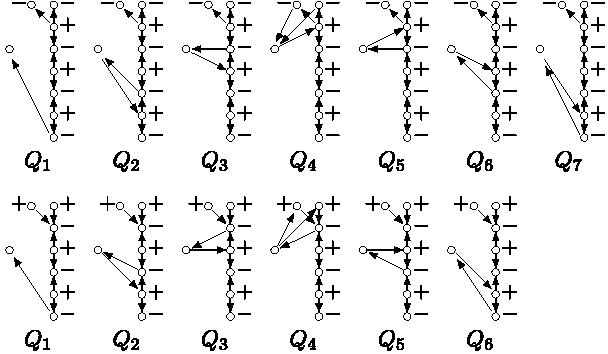
\includegraphics{../assets/2820/Nakanishi-Fig2.pdf}}
\caption{The quiver $Q_{n}(\mathrm{SG})$  for $n=8$
(upper) and for $n=7$ (lower),
where, except for the leftmost vertex of each quiver $Q_i$,
 all the  vertices in the same position
 in  $n-1$ quivers $Q_1,\dots,Q_{n-1}$ are
identif\/ied.}
\label{fig:quiverG}
\end{figure}

Recall that a {\em quiver\/} is an oriented graph,
namely, it consists of the vertices and the arrows
connecting them.
With each $n \geq 4$ we associate
 a quiver $Q_{n}(\mathrm{SG})$ as below.
First, as rather general examples, the cases $n=8$ and $n=7$ are given in
 Fig.~\ref{fig:quiverG},
where, except for the leftmost vertex of each quiver $Q_i$,
 all the  vertices in the same position
 in  $n-1$ quivers $Q_1,\dots,Q_{n-1}$ are
identif\/ied.
For a general $n$,  the quiver $Q_{n}(\mathrm{SG})$ is def\/ined
by naturally extending these examples.
Namely, we consider $n-1$ quivers $Q_1,\dots, Q_{n-1}$,
whose vertices are naturally identif\/ied with
the vertices of the graph $X_n$ in Fig.~\ref{fig:X}.
(The leftmost vertex corresponds to the vertex~$1$ in~$X_n$.)
The arrows are put in $Q_i$ as clearly indicated by the examples
in Fig.~\ref{fig:quiverG}.
Note that the pattern of arrows slightly
depends on the parity of~$n$.
Then, except for the leftmost vertex of each quiver~$Q_i$,
 all the  vertices in the same position
 in  $n-1$ quivers $Q_1,\dots,Q_{n-1}$ are
identif\/ied.
Also we assign the property $+/-$
to  each vertex, except for the leftmost one in each~$Q_i$,
 as in Fig.~\ref{fig:quiverG}.

Let us choose  the index set $\mathbf{I}$
of the vertices of $Q_{n}(\mathrm{SG})$
so that $\mathbf{i}=(i,1)\in \mathbf{I}$ represents
the leftmost vertex in $Q_i$ for $i=1,\dots,n-1$,
 and $\mathbf{i}=(n,i')\in \mathbf{I}$ represents
the vertex $i'=2,\dots,n+1$ in any quiver $Q_i$
under the natural
identif\/ication with $X_n$.
Thus, $i=1,\dots,n$; and $i'=1$ if $i\neq n$
and $i'=2,\dots,n+1$ if $i=n$.

Let $\mathbf{I}_+$
(resp.\ $\mathbf{I}_-$)
denote the set of the vertices $\mathbf{i}\in \mathbf{I}$ with
property  $+$ (resp.\  $-$).
We def\/ine composite mutations (Appendix~\ref{sec:groc}(ii)--(v)),
\begin{gather*}
%\label{eq:mupm2}
\mu_+=\prod_{\mathbf{i}\in\mathbf{I}_+}
\mu_{\mathbf{i}},
\qquad
\mu_-=\prod_{\mathbf{i}\in\mathbf{I}_-}
\mu_{\mathbf{i}}.
\end{gather*}
Note that they do not depend on the order of the product.

For a permutation $\sigma$ of $\{1,\dots,n-1 \}$,
let $\tilde{\sigma}$ be the permutation of
$\mathbf{I}$ such that
$\tilde{\sigma}(i,1)=(\sigma(i),1)$ for $i\neq n$
and $\tilde{\sigma}(n,i')=(n,i')$.
Let $\tilde{\sigma}(Q_{n}(\mathrm{SG}))$
denote the
quiver induced from $Q_{n}(\mathrm{SG})$
 by~$\tilde{\sigma}$.
Namely, if there is an arrow
 $\mathbf{i}\rightarrow
\mathbf{j}$ in $Q_{n}(\mathrm{SG})$,
then, there is an arrow
$\tilde{\sigma}(\mathbf{i})
\rightarrow
\tilde{\sigma}(\mathbf{j})
$
in  $\tilde{\sigma}(Q_{n}(\mathrm{SG}))$.

\begin{Lemma}
\label{lem:GQmut}
Let $Q(0):=Q_{n}(\mathrm{SG})$.
We have the following periodic sequence of mutations of quivers:
\begin{gather}
% 1st
Q(0)
\mathop{\longleftrightarrow}^{{\mu_+} \mu_{(1,1)}}
 Q(1)
\mathop{\longleftrightarrow}^{\mu_-}
Q(2)
\displaystyle
\mathop{\longleftrightarrow}^{\mu_+ \mu_{(2,1)}}
Q(3)
\displaystyle
\mathop{\longleftrightarrow}^{\mu_-}
Q(4)
\nonumber\\
\hphantom{Q(0)
\mathop{\longleftrightarrow}^{{\mu_+} \mu_{(1,1)}}}{}
\mathop{\longleftrightarrow}^{\mu_+\mu_{(3,1)}}
\ \cdots\
\displaystyle
\mathop{\longleftrightarrow}^{\mu_+\mu_{(n-1,1)}}
Q(2n-3)
\displaystyle
\mathop{\longleftrightarrow}^{\mu_-}
Q(2n-2)=Q(0),\label{eq:GB2}
\end{gather}
where the quiver $Q(2p)$ $(p=1,\dots,n-2)$ is given by
\begin{gather}
\label{eq:Q2p}
Q(2p)=
\tilde{\sigma}^p(Q(0)),
\qquad
\sigma=\left(
\begin{matrix}
1&2&\dots &n-2 &n-1\\
2&3& \dots&n-1& 1\\
\end{matrix}
\right).
\end{gather}
\end{Lemma}

\begin{Example}
The mutation sequence
 \eqref{eq:GB2} for $n=6$ is explicitly given
in Fig.~\ref{fig:labelxG1}.
\begin{figure}[t]
\centerline{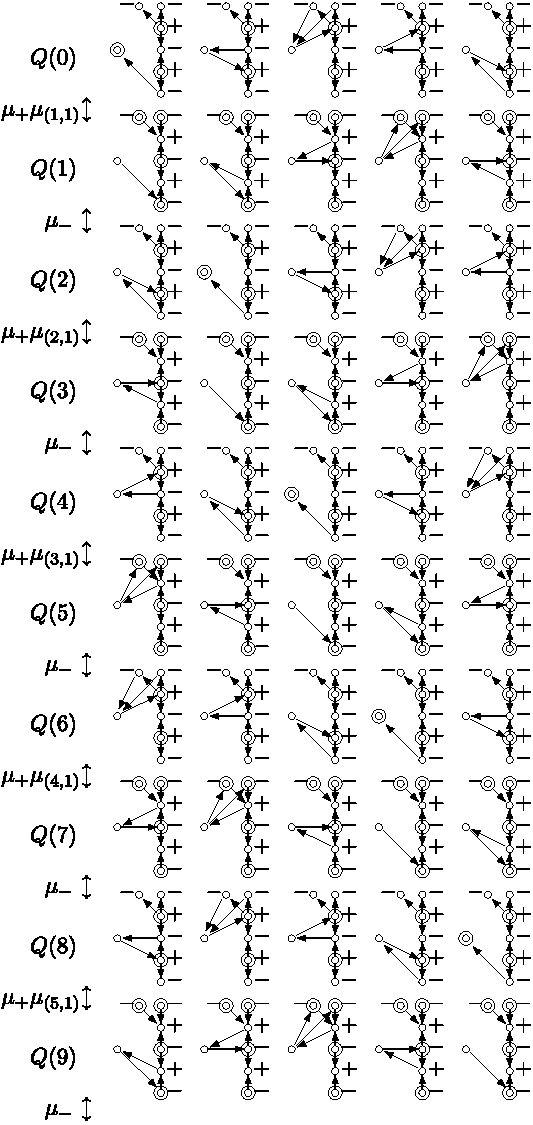
\includegraphics{../assets/2820/Nakanishi-Fig3.pdf}}

\caption{The mutation sequence of the quiver $Q_{n}(\mathrm{SG})$
in~\eqref{eq:GB2} for $n=6$.
The encircled vertices correspond to
the mutation points
$(\mathbf{i},u): \mathbf{p}_+$ in the forward direction.}
\label{fig:labelxG1}
\end{figure}
\end{Example}



\subsection{Embedding maps}
Let
 $B=B_{n}(\mathrm{SG})$
be the skew-symmetric matrix corresponding
to the quiver $Q_{n}(\mathrm{SG})$ (Appendix~\ref{sec:groc}(iii)).
Let $\mathcal{A}(B,x,y)$
be the cluster algebra
 with coef\/f\/icients
in the universal
semif\/ield
$\mathbb{P}_{\mathrm{univ}}(y)$ (Appendix~\ref{sec:groc}(vi)).



In view of Lemma~\ref{lem:GQmut}
we set $x(0)=x$, $y(0)=y$ and def\/ine
clusters $x(u)=(x_{\mathbf{i}}(u))_{\mathbf{i}\in \mathbf{I}}$
 ($u\in \mathbb{Z}$)
 and coef\/f\/icient tuples $y(u)=(y_\mathbf{i}(u))_{\mathbf{i}\in \mathbf{I}}$
 ($u\in \mathbb{Z}$)
by the sequence of mutations
\begin{gather}
% 1st
\cdots
\ \mathop{\longleftrightarrow}^{\mu_-}\
(B(0),x(0),y(0))
\ \mathop{\longleftrightarrow}^{\mu_+
\mu_{(1,1)}}\
(B(1),x(1),y(1))\nonumber\\
\phantom{\cdots}{} \ \mathop{\longleftrightarrow}^{\mu_-}\
\cdots
\ \mathop{\longleftrightarrow}^{\mu_-}\
(B(2n-2),x(2n-2),y(2n-2))
\ \mathop{\longleftrightarrow}^{\mu_+
\mu_{(1,1)}}\
\cdots,\label{eq:Gmutseq}
\end{gather}
where $B(u)$ is the skew-symmetric matrix corresponding to
$Q(u)$.

For  $(\mathbf{i},u)\in
 \mathbf{I}\times \mathbb{Z}$,
we set the parity condition $\mathbf{p}_+$ by
\begin{gather}
\label{eq:GQparity}
\mathbf{p}_+: \
\begin{cases}
 \mathbf{i}\in
\mathbf{I}_+ \sqcup
\{(j+1,1)\},
& u\equiv 2j
\ (j=0,1,\dots,n-2),\\
 \mathbf{i}\in
\mathbf{I}_-,
& \mbox{$u$: odd},
\end{cases}
\end{gather}
where $\equiv$ is modulo $(2n-2)\mathbb{Z}$.
We def\/ine the condition $\mathbf{p}_-$
by $(\mathbf{i},u):\mathbf{p}_- \Longleftrightarrow
(\mathbf{i},u-1):\mathbf{p}_+$.
Plainly speaking,
each $(\mathbf{i},u):\mathbf{p}_+$
(resp.\ $(\mathbf{i},u):\mathbf{p}_-$)
is a mutation point of~\eqref{eq:Gmutseq} in the forward
(resp. backward) direction of~$u$.
See Fig.~\ref{fig:labelxG1}.

\begin{Lemma}
\label{lem:gmap}
Below $\equiv$ means the equivalence modulo $(2n-2)\mathbb{Z}$.

\begin{enumerate}\itemsep=0pt
\item[$(i)$]
The map
\begin{gather*}
g:  \ \mathcal{I}_{n+} \rightarrow
\{ (\mathbf{i},u)\in \mathbf{I}\times \mathbb{Z} \mid
(\mathbf{i},u): \mathbf{p}_+
\}, \\
\phantom{g: \ } \ (i,u-d_i) \mapsto
\begin{cases}
((j+1,1),u), & i= 1; \
u \equiv 2j
\ (j=0,1,\dots,n-2),\\
((n,i),u), & i=2,\dots,n+1
\end{cases}
\end{gather*}
is a bijection.

\item[$(ii)$]
The map
\begin{gather*}
g': \  \mathcal{I}'_{n+} \rightarrow
\{ (\mathbf{i},u)\in \mathbf{I}\times \mathbb{Z} \mid
 (\mathbf{i},u): \mathbf{p}_+
\}, \\
\phantom{g': \ }{} \  (i,u) \mapsto
\begin{cases}
((j+1,1),u), & i= 1;\
u\equiv 2j
\ (j=0,1,\dots,n-2), \\
((n,i),u), &  i=2,\dots,n+1
\end{cases}
\end{gather*}
is a bijection.
\end{enumerate}
\end{Lemma}

Based on Lemma \ref{lem:gmap},
we introduce alternative notations
$\tilde{x}_i(u-d_i):=x_{\mathbf{i}}(u)$
for $(i,u-d_i)\in \mathcal{I}_{n+}$
with $(\mathbf{i},u)=g((i,u-d_i))$
and
$y_i(u):=y_{\mathbf{i}}(u)$
for $(i,u)\in \mathcal{I}'_{n+}$
with $(\mathbf{i},u)=g'((i,u))$,
respectively,
which turn out to be useful.

 Let $\mathcal{A}(B,x)$ be the cluster algebra
with trivial coef\/f\/icients, where $(B,x)$ is
the initial seed
and the coef\/f\/icient semif\/ield
is the {\em trivial semifield\/}
 $\mathbf{1}=\{1\}$ (Appendix~\ref{sec:groc}(i)).
Let $\pi_{\mathbf{1}}:
\mathbb{P}_{\mathrm{univ}}(y)\rightarrow
\mathbf{1}$, $y_{\mathbf{i}}\mapsto 1$ be the projection.
Let $[x_{\mathbf{i}}(u)]_{\mathbf{1}}$
denote the image of $x_{\mathbf{i}}(u)$
 by the algebra homomorphism
$\mathcal{A}(B,x,y)\rightarrow \mathcal{A}(B,x)$
 induced from $\pi_{\mathbf{1}}$.
It is called the {\em trivial evaluation}.




The following lemma follows from the exchange relation
of
cluster variables \eqref{eq:clust}
and the property of the sequence \eqref{eq:GB2}
 observed in Fig.~\ref{fig:labelxG1}.

\begin{Lemma}
\label{lem:Gx2}
Let $G_+$ and $G_-$ be the ones in \eqref{eq:Yuni} and \eqref{eq:Tuni}.
The family $\{\tilde{x}_i(u)
\mid (i,u)\in \mathcal{I}_{n+}\}$
satisfies a system of relations
\begin{gather}
\tilde{x}_i\left(u-d_i\right)
\tilde{x}_i\left(u+d_i\right)
 =
\frac{y_i(u)}{1+y_i(u)}
\prod_{(j,v)\in \mathcal{I}_{n+}}
\tilde{x}_j(v)^{G_+(i,u;j,v)}
\nonumber\\
\phantom{\tilde{x}_i\left(u-d_i\right)
\tilde{x}_i\left(u+d_i\right)
 =}{}
+
\frac{1}{1+y_i(u)}
\prod_{(j,v)\in \mathcal{I}_{n+}}
\tilde{x}_j(v)^{G_-(i,u;j,v)},\label{eq:xy1}
\end{gather}
where $(i,u)\in \mathcal{I}'_{n+}$.
In particular,
the family $\{ [\tilde{x}_i(u)]_{\mathbf{1}}
\,|\, (i,u)\in \mathcal{I}_{n+}\}$
satisfies the T-system $\mathbb{T}_{n}(\mathrm{SG})$
in $\mathcal{A}(B,x)$
by replacing $T_i(u)$ with $[\tilde{x}_i(u)]_{\mathbf{1}}$.
\end{Lemma}

\begin{Example}
Consider the case $n=6$ in Fig.~\ref{fig:labelxG1}.
Let us consider the mutation at the vertex~$(1,1)$ in $Q(0)$,
to which  the variable $\tilde{x}_1(-5)$ is attached.
The next time~$(1,1)$ is mutated is in~$Q(10)$,
where~$\tilde{x}_1(5)$ is attached.
Meanwhile, the only vertex connected to~$(1,1)$ in~$Q(0)$ is~$(6,2)$,
and the  variable attached to $(6,2)$ in $Q(0)$ is equal to
the variable  $\tilde{x}_2(0)$ attached to~$(6,2)$ in~$Q(1)$.
Taking account of the directions of the arrows,
we have the  relation
\begin{align*}
\tilde{x}_1(-5)\tilde{x}_1(5)=
\frac{y_1(0)}{1+y_1(0)} \tilde{x}_2(0)
+ \frac{1}{1+y_1(0)} ,
\end{align*}
which agrees with
\eqref{eq:T1} and
\eqref{eq:xy1}.
Similarly, consider the mutation at the vertex $(6,2)$ in $Q(1)$,
to which  the variable $\tilde{x}_2(0)$ is attached.
The next time $(6,2)$ is mutated is in $Q(3)$,
where $\tilde{x}_2(2)$ is attached.
Meanwhile, the vertices connected to $(6,2)$ in $Q(1)$
are $(1,1)$, $(2,1)$, and $(6,3)$,
and the  variable attached to them are equal to
$\tilde{x}_1(5)$, $\tilde{x}_1(-3)$, and $\tilde{x}_3(1)$, respectively.
Taking account of the directions of the arrows,
we have the relation
\begin{align*}
\tilde{x}_2(0)\tilde{x}_2(2)=
\frac{y_2(1)}{1+y_2(1)} \tilde{x}_1(-3)\tilde{x}_1(5)
+ \frac{1}{1+y_2(1)} \tilde{x}_3(1).
\end{align*}
As the last example,
consider the mutation at the vertex $(6,6)$ in $Q(1)$,
to which  the va\-riab\-le~$\tilde{x}_6(0)$ is attached.
The next time $(6,6)$ is mutated is in $Q(3)$,
where $\tilde{x}_6(2)$ is attached.
Meanwhile, the vertices connected to $(6,6)$ in $Q(1)$
are $(4,1)$ and $(6,5)$,
and the  variable attached to them are equal to
$\tilde{x}_1(1)$ and  $\tilde{x}_5(1)$, respectively.
Taking account of the directions of the arrows,
we have the relation
\[
\tilde{x}_6(0)\tilde{x}_6(2)=
\frac{y_6(1)}{1+y_6(1)} \tilde{x}_1(1)
+ \frac{1}{1+y_6(1)} \tilde{x}_5(1).
\]
The other cases can be checked in similar manners.
\end{Example}

\begin{Definition}
\label{def:T-sub}
The {\em T-subalgebra
$\mathcal{A}_T(B,x)$
of ${\mathcal{A}}(B,x)$
associated with the sequence \eqref{eq:Gmutseq}}
is the subring of
${\mathcal{A}}(B,x)$
generated by
$[x_{\mathbf{i}}(u)]_{\mathbf{1}}$
($(\mathbf{i},u)\in \mathbf{I}\times \mathbb{Z}$),
or equivalently,
generated by
$[\tilde{x}_{i}(u)]_{\mathbf{1}}$
($(i,u)\in \mathcal{I}_{n+}$).
\end{Definition}

By Lemma \ref{lem:Gx2}, we have the following embedding.
\begin{Theorem}
\label{thm:GTiso}
The ring $\EuScript{T}^{\circ}_{n}(\mathrm{SG})_+$ is isomorphic to
$\mathcal{A}_T(B,x)$ by the correspondence
$T_i(u)\mapsto [\tilde{x}_i(u)]_{\mathbf{1}}$.
\end{Theorem}



The {\em coefficient group $\mathcal{G}(B,y)$
associated with $\mathcal{A}(B,x,y)$}
is the multiplicative subgroup of
the semif\/ield $\mathbb{P}_{\mathrm{univ}}(y)$ generated by all
the coef\/f\/icients $y_{\mathbf{i}}'$ of $\mathcal{A}(B,x,y)$
together with $1+y_{\mathbf{i}}'$.

The following lemma follows from the exchange relation of
coef\/f\/icients \eqref{eq:coef} and the property of the sequence
\eqref{eq:GB2}.


\begin{Lemma}
\label{lem:Gy2}
The family $\{ y_i(u)
\mid (i,u)\in \mathcal{I}'_{n+}\}$
satisfies the Y-system $\mathbb{Y}_{n}(\mathrm{SG})$
by replacing $Y_i(u)$ with $y_i(u)$.
\end{Lemma}

\begin{Example}
Consider the case $n=6$ in Fig.~\ref{fig:labelxG1}.
Let us consider the mutation at the vertex~$(1,1)$ in $Q(0)$,
to which  the variable $y_1(0)$ is attached.
The next time~$(1,1)$ is mutated is in~$Q(10)$,
where $y_1(10)$ is attached.
Meanwhile, between $u=0$ and $u=10$,
the vertices connected to $(1,1)$ in~$Q(u)$ and mutated
are
$(6,2)$ at $u=1,9$, $(6,3)$ at $u=2,8$, $(6,4)$ at $u=3,7$,
$(6,5)$ at $u=4,6$, and  $(6,6)$ and $(6,7)$ at~$u=5$,
Taking account of the directions of the arrows,
we have the relation
\begin{gather*}
y_1(0)y_1(10)=
(1+y_2(1))(1+y_2(9))(1+y_3(2))(1+y_3(8)) (1+y_4(3))\\
\phantom{y_1(0)y_1(10)=}{} \times (1+y_4(7))
(1+ y_5(4))(1+y_5(6)) (1+y_6(5))(1+y_7(5)),
\end{gather*}
which agrees with
\eqref{eq:Y1}.
Similarly, consider the mutation at the vertex $(6,2)$ in $Q(1)$,
to which  the variable $y_2(1)$ is attached.
The next time $(6,2)$ is mutated is in $Q(3)$,
where $y_2(3)$ is attached.
Meanwhile, between $u=1$ and $u=3$,
the vertices connected to $(6,2)$ in $Q(u)$ and mutated
are~$(2,1)$ and~$(6,3)$ at $u=2$.
Taking account of the directions of the arrows,
we have the relation
\[
y_2(1)y_2(3) =
\frac{(1+y_1(2))}{1+y_3(2)^{-1}}.
\]
As the last example, consider the mutation at the vertex $(6,6)$ in $Q(1)$,
to which  the variable~$y_6(1)$ is attached.
The next time $(6,6)$ is mutated is in $Q(3)$,
where $y_6(3)$ is attached.
Meanwhile, between $u=1$ and $u=3$,
the only vertex connected to $(6,6)$ in $Q(u)$ and mutated
is  $(6,5)$ at~$u=2$.
Taking account of the directions of the arrows,
we have the relation
\[
y_6(1)y_6(3) =
\frac{1}{1+y_5(2)^{-1}}.
\]
The other cases can be checked in similar manners.
\end{Example}

\begin{Definition}
The {\em Y-subgroup
$\mathcal{G}_Y(B,y)$
of $\mathcal{G}(B,y)$
associated with the sequence \eqref{eq:Gmutseq}}
is the subgroup of
$\mathcal{G}(B,y)$
generated by
$y_{\mathbf{i}}(u)$
($(\mathbf{i},u)\in \mathbf{I}\times \mathbb{Z}$)
and $1+y_{\mathbf{i}}(u)$
($(\mathbf{i},u):\mathbf{p}_+$ or $\mathbf{p}_-$),
or equivalently,
generated by
$y_i(u)$ and $1+y_i(u)$
($(i,u)\in \mathcal{I}'_{n+}$).
\end{Definition}

By Lemma \ref{lem:Gy2}, we have the following embedding.
\begin{Theorem}
\label{thm:GYiso}
The group $\EuScript{Y}^{\circ}_{n}(\mathrm{SG})_+$ is isomorphic to
$\mathcal{G}_Y(B,y)$ by the correspondence
$Y_i(u)\mapsto y_i(u)$
and $1+Y_i(u)\mapsto 1+y_i(u)$.
\end{Theorem}


\section{Proof of
Theorems \ref{thm:Yperiod}, \ref{thm:dilog},
and \ref{thm:Tperiod}}
\label{sec:proofSG}

In this section we prove
Theorems \ref{thm:Yperiod}, \ref{thm:dilog},
and \ref{thm:Tperiod}
using the method of \cite{Nakanishi09,Inoue10a}.


Let $y=y(0)$ be the initial coef\/f\/icient tuple
of the cluster algebra $\mathcal{A}(B,x,y)$
with $B=B_{n}(\mathrm{SG})$ in the previous section.
Let
$\mathbb{P}_{\mathrm{trop}}(y)$ be
the {\em tropical semifield} for $y$ (Appendix~\ref{sec:groc}(i)).
Let $\pi_{\mathbf{T}}:
\mathbb{P}_{\mathrm{univ}}(y)\rightarrow
\mathbb{P}_{\mathrm{trop}}(y)$, $y_{\mathbf{i}}\mapsto
y_{\mathbf{i}}$ be the projection.
Let $[y_{\mathbf{i}}(u)]_{\mathbf{T}}$
and $[\mathcal{G}_Y(B,y)]_{\mathbf{T}}$
denote the images of $y_{\mathbf{i}}(u)$
and $\mathcal{G}_Y(B,y)$
by the multiplicative group
 homomorphism induced from $\pi_{\mathbf{T}}$, respectively.
They are called the {\em tropical evaluations},
and the resulting relations in
the group $[\mathcal{G}_Y(B,y)]_{\mathbf{T}}$
are called the {\em tropical Y-system}.
They are f\/irst studied in~\cite{Fomin03b}
for cluster algebras of f\/inite types.

We say a (Laurent) monomial $m=\prod_{\mathbf{i}\in \mathbf{I}}
y_{\mathbf{i}}^{k_{\mathbf{i}}}$
is {\em positive} (resp. {\em negative})
if $m\neq 1$ and $k_{\mathbf{i}}\geq 0$
(resp. $k_{\mathbf{i}}\leq 0$)
for any $\mathbf{i}$.
It is known that every monomial $[y_{\mathbf{i}}(u)]_{\mathbf{T}}$
is either positive or negative by \cite[Proposition 5.6]{Fomin07}
and \cite[Theorem 1.7]{Derksen10}.

The next `tropical mutation rule' for $[y_{\mathbf{i}}(u)]_{\mathbf{T}}$
is general and  useful.
\begin{Lemma}
\label{lem:mutation}
Suppose that $y''$ is the coefficient tuple obtained from
the mutation of another coefficient tuple $y'$ at $\mathbf{k}$
with mutation matrix $B'$. Then, for any $\mathbf{i}\neq \mathbf{k}$,
we have the rule:
\begin{enumerate}\itemsep=0pt
\item[$(i)$] $[y''_{\mathbf{i}}]_{\mathbf{T}} =
 [y'_{\mathbf{i}}]_{\mathbf{T}}[y'_{\mathbf{k}}]_{\mathbf{T}}$
 if one of the following conditions holds:
\begin{enumerate}\itemsep=0pt
\item[$(a)$] $B'_{\mathbf{k}\mathbf{i}}> 0$,
 and $[y'_{\mathbf{k}}]_{\mathbf{T}}$ is
positive;
\item[$(b)$]  $B'_{\mathbf{k}\mathbf{i}}< 0$,
 and $[y'_{\mathbf{k}}]_{\mathbf{T}}$ is
negative.
\end{enumerate}
\item[$(ii)$]
$[y''_{\mathbf{i}}]_{\mathbf{T}} =
 [y'_{\mathbf{i}}]_{\mathbf{T}}$
 if one of the following conditions holds:
\begin{enumerate}\itemsep=0pt
\item[$(a)$] $B'_{\mathbf{k}\mathbf{i}}=0$;

\item[$(b)$]
 $B'_{\mathbf{k}\mathbf{i}}> 0$,
 and $[y'_{\mathbf{k}}]_{\mathbf{T}}$ is
 negative;
\item[$(c)$] $B'_{\mathbf{k}\mathbf{i}}< 0$,
 and $[y'_{\mathbf{k}}]_{\mathbf{T}}$ is
 positive.
 \end{enumerate}
 \end{enumerate}
\end{Lemma}
\begin{proof}
This is an immediate consequence of the exchange relation
\eqref{eq:coef} and \eqref{eq:trop}.
\end{proof}


The following properties
of the tropical Y-system are crucial.

\begin{Proposition}
\label{prop:lev2}
 For
$[\mathcal{G}_Y(B,y)]_{\mathbf{T}}$
with $B=B_{n}(\mathrm{SG})$, the following facts hold.

\begin{enumerate}\itemsep=0pt
\item[$(i)$]  For $0 \le u < 4n-2$,
the  monomial $[y_{\mathbf{i}}(u)]_{\mathbf{T}}$
$((\mathbf{i},u):\mathbf{p}_+)$
is negative if and only if $u$ takes the following values.
\[
\begin{cases}
2n-2 \leq u < 4n-2 &
\quad\mbox{\rm for $\mathbf{i}=(1,1),\dots,(n-1,1),(n,2)$},\\
u=2n-2,2n-1, 4n-4, 4n-3 &
\quad\mbox{\rm for $\mathbf{i}=(n,3),\dots,(n,n+1)$}.
\end{cases}
\]
$($Note that for each $\mathbf{i}$, $u$ takes only a part
of the list due to the condition $(\mathbf{i},u):\mathbf{p}_+.)$
\item[$(ii)$]
 We have $[y_{\mathbf{i}}(4n-2)]_{\mathbf{T}}
=y_{\tau^{-1}(\mathbf{i})}$,
where $\tau$ is a bijection $\mathbf{I} \rightarrow
\mathbf{I}$ defined by
\begin{gather*}
(i,1)   \mapsto (\sigma(i),1),
\qquad i=1,\dots,n-1,\\
(n,i')   \mapsto
\begin{cases}
(n,i'),& i'=2,\dots,n-1,\\
(n,n+1),& i'=n,\\
(n,n),& i'=n+1
\end{cases}
\end{gather*}
and $\sigma$ is the permutation in~\eqref{eq:Q2p}.

\item[$(iii)$] The number $N_-$ of the negative monomials
$[y_{\mathbf{i}}(u)]_{\mathbf{T}}$ for $(\mathbf{i},u):\mathbf{p}_+$
in the region $0\leq u < 4n-2$ is $4n-2$.
\end{enumerate}
\end{Proposition}



\begin{proof}
$(i)$ Let us factorize $[y_{\mathbf{i}}(u)]_{\mathbf{T}}
=[y_{\mathbf{i}}(u)]'_{\mathbf{T}}
[y_{\mathbf{i}}(u)]''_{\mathbf{T}}$,
where
 $[y_{\mathbf{i}}(u)]'_{\mathbf{T}}$ is a monomial
in $y_{(i,1)}$ ($i=1,\dots,n-1$)
while
 $[y_{\mathbf{i}}(u)]''_{\mathbf{T}}$ is a monomial
in $y_{(n,i')}$ ($i'=2,\dots,n+1$).
One can independently study
$[y_{\mathbf{i}}(u)]'_{\mathbf{T}}$ and
$[y_{\mathbf{i}}(u)]''_{\mathbf{T}}$.
The claim  (i) follows from the following results,
which  are proved inductively on $u$
by Lemma \ref{lem:mutation} and the results of
\cite{Fomin03b,Fomin07}.

$(a)$ $[y_{\mathbf{i}}(u)]'_{\mathbf{T}}$ part.
This part is easier.
All the monomials $[y_{\mathbf{i}}(u)]'_{\mathbf{T}}$
 which are not 1 for $(\mathbf{i},u):\mathbf{p}_+$
in the region $0 \leq u < 4n-2$ are as follows.
We have $[y_{(i,1)}(2i-2)]'_{\mathbf{T}}=y_{(i,1)}$
$(i=1,\dots,n-1)$,
and also
\begin{alignat}{3}
& [y_{(1,1)}(2n-2)]'_{\mathbf{T}}=y_{(1,1)}^{-1},\qquad &&
[y_{(n,2)}(2n-1)]'_{\mathbf{T}}=y_{(1,1)}^{-1},&\notag\\
& [y_{(2,1)}(2n)]'_{\mathbf{T}}=y_{(1,1)}^{-1}y_{(2,1)}^{-1},\qquad &&
[y_{(n,2)}(2n+1)]'_{\mathbf{T}}=y_{(2,1)}^{-1},&\notag\\
\label{eq:y'part}
& [y_{(3,1)}(2n+2)]'_{\mathbf{T}}=y_{(2,1)}^{-1}y_{(3,1)}^{-1},\qquad &&
[y_{(n,2)}(2n+3)]'_{\mathbf{T}}=y_{(3,1)}^{-1},&\\
&\qquad \vdots & &\qquad \vdots & \notag\\
& [y_{(n-1,1)}(4n-6)]'_{\mathbf{T}}=y_{(n-2,1)}^{-1}y_{(n-1,1)}^{-1},\qquad &&
[y_{(n,2)}(4n-5)]'_{\mathbf{T}}=y_{(n-1,1)}^{-1},&\notag\\
& [y_{(1,1)}(4n-4)]'_{\mathbf{T}}=y_{(n-1,1)}^{-1}.&&& \notag
\end{alignat}

$(b)$  $[y_{\mathbf{i}}(u)]''_{\mathbf{T}}$ part.
Below we list all the monomials $[y_{\mathbf{i}}(u)]''_{\mathbf{T}}$
which are not 1 for $(\mathbf{i},u):\mathbf{p}_+$
in the region $0 \leq u < 4n-2$.
We separate the region $0 \leq u < 4n-2$ into four parts
corresponding to the decomposition
$4n-2=(2n-2)+2+(2n-4)+2$,
where $2n-2$ and $2n-4$ are the Coxeter numbers
of $D_{n}$ and $D_{n-1}$.


Region I: $0\leq u < 2n-2$.
All the  monomials
$[y_{(n,i')}(u)]''_{\mathbf{T}}$ ($i'=2,\dots,n+1$)
 for $(\mathbf{(n,i')},u):\mathbf{p}_+$
are identif\/ied with
the {\em positive roots of $D_n$} as in
\cite[Proposition 10.7]{Fomin07};
therefore, they are positive.
Here, $D_{n}$ is identif\/ied with the subgraph of $X_n$
consisting of vertices $2, \dots, n+1$.


Region II: $u=2n-2$, $2n-1$.
We have, for even $n$,
\begin{gather*}
[y_{(n,i')}(2n-2)]''_{\mathbf{T}} =y_{(n,i')}^{-1},\qquad  i'=3,5,\dots,n-1 ,\nonumber\\
[y_{(n,i')}(2n-1)]''_{\mathbf{T}} =y_{(n,i')}^{-1},\qquad  i'=2,4,\dots,n,n+1 ,%\label{eq:yt1}
\end{gather*}
and, for odd $n$,
\begin{gather*}
[y_{(n,i')}(2n-2)]''_{\mathbf{T}} =y_{(n,i')}^{-1}, \qquad  i'=3,5,\dots,n-2 ,\nonumber\\
[y_{(n,n)}(2n-2)]''_{\mathbf{T}} =y_{(n,n+1)}^{-1},
\qquad [y_{(n,n+1)}(2n-2)]''_{\mathbf{T}}=y_{(n,n)}^{-1},\nonumber\\
[y_{(n,i')}(2n-1)]''_{\mathbf{T}} =y_{(n,i')}^{-1},\qquad i'=2,4,\dots,n-1.%\label{eq:yt4}
\end{gather*}

Region III: $2n \leq u < 4n-4$.
All the  monomials
$[y_{(n,i')} (u)]''_{\mathbf{T}}$ ($i'=3,\dots,n+1$)
 for $((n,i'),u):\mathbf{p}_+$
are  identif\/ied with
the {\em positive roots of $D_{n-1}$},
therefore, they are positive.
Here, $D_{n-1}$ is identif\/ied with the subgraph of $X_n$
consisting of vertices $3, \dots, n+1$.

Region IV: $u=4n-4$, $4n-3$. We have, for even $n$,
\begin{gather}
[y_{(n,i')}(4n-4)]''_{\mathbf{T}} =y_{(n,i')}^{-1}, \qquad i'=3,5,\dots,n-1,\nonumber\\
[y_{(n,i')}(4n-3)]''_{\mathbf{T}} =y_{(n,i')}^{-1}, \qquad i'=2,4,\dots,n-2,\nonumber\\
[y_{(n,n)}(4n-3)]''_{\mathbf{T}} =y_{(n,n+1)}^{-1},
\qquad [y_{(n,n+1)}(4n-3)]''_{\mathbf{T}}=y_{(n,n)}^{-1},\label{eq:yt3}
\end{gather}
and, for odd $n$,
\begin{gather}
[y_{(n,i')}(4n-4)]''_{\mathbf{T}} =y_{(n,i')}^{-1}, \qquad  i'=3,5,\dots,n-2 ,\nonumber\\
[y_{(n,n)}(4n-4)]''_{\mathbf{T}} =y_{(n,n+1)}^{-1},
\qquad [y_{(n,n+1)}(4n-4)]''_{\mathbf{T}}=y_{(n,n)}^{-1},\nonumber\\
[y_{(n,i')}(4n-3)]''_{\mathbf{T}} =y_{(n,i')}^{-1},\qquad i'=2,4,\dots,n-1.\label{eq:yt6}
\end{gather}

Besides, we have the sequences of  monomials
which appear over Regions~III and~IV;
for even~$n$,
\begin{gather}
 [y_{(2,1)}(2n)]''_{\mathbf{T}}=y_{(n,2)}^{-1}y_{(n,3)}^{-1},
\qquad [y_{(3,1)}(2n+2)]''_{\mathbf{T}}=y_{(n,4)}^{-1}y_{(n,5)}^{-1},
\qquad \dots,\nonumber\\
 [y_{(n/2,1)}(3n-4)]''_{\mathbf{T}}=y_{(n,n-2)}^{-1}y_{(n,n-1)}^{-1},\qquad
 [y_{(n/2+1,1)}(3n-2)]''_{\mathbf{T}}=y_{(n,n-1)}^{-1}y_{(n,n)}^{-1}y_{(n,n+1)}^{-1},\nonumber\\
 [y_{(n/2+2,1)}(3n)]''_{\mathbf{T}}=y_{(n,n-3)}^{-1}y_{(n,n-2)}^{-1},\qquad
\dots,\nonumber\\
  [y_{(n-1,1)}(4n-6)]''_{\mathbf{T}}=y_{(n,3)}^{-1}y_{(n,4)}^{-1},
\qquad [y_{(1,1)}(4n-4)]''_{\mathbf{T}}=y_{(n,2)}^{-1},\label{eq:yt2}
\end{gather}
and, for odd $n$, the middle three terms are replaced with
\begin{gather}
 [y_{((n-1)/2,1)}(3n-5)]''_{\mathbf{T}}=y_{(n,n-3)}^{-1}y_{(n,n-2)}^{-1},\nonumber\\
 [y_{((n+1)/2,1)}(3n-3)]''_{\mathbf{T}}=
y_{(n,n-1)}^{-1}y_{(n,n)}^{-1}y_{(n,n+1)}^{-1},\nonumber\\
 [y_{(n+3)/2,1)}(3n-1)]''_{\mathbf{T}}=y_{(n,n-2)}^{-1}y_{(n,n-1)}^{-1}.\label{eq:yt5}
\end{gather}

$(ii)$ They  follow from
\eqref{eq:yt3}--\eqref{eq:yt5}.


$(iii)$ By $(i)$, for each  $\mathbf{i}$
the numbers of the negative monomials
$[y_{\mathbf{i}}(u)]_{\mathrm{T}}$
in the region is~2 for $\mathbf{i}= (1,1)$,
 1 for $\mathbf{i}= (i,1)$ ($i=2,\dots,n-1$),
$n$ for $\mathbf{i}= (n,2)$.
and $2$ for $\mathbf{i}=(n,i')$ ($i'=3,\dots,n+1$).
Summing up, we have $N_-=4n-2$.
\end{proof}

Now we prove
Theorems \ref{thm:Yperiod} and \ref{thm:Tperiod}.
It follows from  a very general theorem
\cite[Theorem 5.1]{Inoue10a}
(based on the work by Plamondon \cite{Plamondon10a,Plamondon10b})
that the cluster variables
$x_{\mathbf{i}}(u)$ and coef\/f\/icients $y_{\mathbf{i}}(u)$
have the same periodicity with
$[y_{\mathbf{i}}(u)]_{\mathbf{T}}$ as in Proposition \ref{prop:lev2}$(ii)$,
namely,
$x_{\mathbf{i}}(4n-2)=x_{\tau^{-1}(\mathbf{i})}$
and
$y_{\mathbf{i}}(4n-2)=y_{\tau^{-1}(\mathbf{i})}$.
It follows that, under the labelling introduced in Lemma
\ref{lem:gmap}, we have
\begin{gather}
\tilde{x}_i(u+4n-2) =\tilde{x}_{\omega(i)}(u),
\qquad (i,u):\mathbf{P}_+,\nonumber\\
y_i(u+4n-2) =y_{\omega(i)}(u),
\qquad (i,u):\mathbf{P}'_+,\label{eq:xperiod}
\end{gather}
where $\omega$ is the one in Theorem~\ref{thm:Yperiod}$(i)$.
Then, thanks to the isomorphisms
in Theorems~\ref{thm:GTiso} and~\ref{thm:GYiso},
and also by the isomorphisms
$\EuScript{T}^{\circ}_{n}(\mathrm{SG})_+
\simeq
\EuScript{T}^{\circ}_{n}(\mathrm{SG})_-
$
and
$\EuScript{Y}^{\circ}_{n}(\mathrm{SG})_+
\simeq
\EuScript{Y}^{\circ}_{n}(\mathrm{SG})_-
$,
we obtain
Theorems~\ref{thm:Yperiod} and~\ref{thm:Tperiod}.
\setcounter{section}{7}
\setcounter{subsection}{3}
\setcounter{subsubsection}{0}
\setcounter{Theorem}{11}
\setcounter{equation}{5}
% Original source lines 3381--3555
\appendix
\section{Cluster algebras}

\label{sec:groc}

Here we collect basic def\/initions for cluster algebras
to f\/ix the convention and notation,
mainly following~\cite{Fomin07}.
For further necessary def\/initions and information
for cluster algebras, see~\cite{Fomin07}.

Let $I$ be a f\/inite index set throughout the appendix.

{\bf (i) Semif\/ield.}
A {\em semifield\/} $(\mathbb{P},\oplus, \cdot)$
is an Abelian multiplicative group
endowed with a binary
operation of addition $\oplus$ which is commutative,
associative, and distributive with respect to the
multiplication in $\mathbb{P}$.
The following three examples are important.


(a) {\em  Trivial semifield.}
The {\em trivial semifield\/}
$\mathbf{1}=\{\mathrm{1}\}$
consists of the multiplicative identity element $1$
with $1\oplus 1 = 1$.

\par
(b) {\em Universal semifield.}
For an $I$-tuple of variables $y=(y_i)_{i\in I}$,
the {\em universal semifield\/}
$\mathbb{P}_{\mathrm{univ}}(y)$
consists of  all the rational functions
of the form
$P(y)/Q(y)$  (subtraction-free  rational expressions),
where $P(y)$ and $Q(y)$ are the nonzero polynomials
 in $y_i$'s with {\em nonnegative\/} integer coef\/f\/icients.
The multiplication and the addition
are given by the usual ones of rational functions.


(c) {\em Tropical semifield.}
For an $I$-tuple of variables $y=(y_i)_{i\in I}$,
the {\em tropical semifield\/}
$\mathbb{P}_{\mathrm{trop}}(y)$
is the Abelian multiplicative group freely generated by
the variables  $y_i$'s endowed with the addition~$\oplus$
\begin{gather}
\label{eq:trop}
\prod_i y_i^{a_i}\oplus
\prod_i y_i^{b_i}
=
\prod_i y_i^{\min(a_i,b_i)}.
\end{gather}



{\bf (ii)  Mutations of matrix and quiver.}
An integer matrix
$B=(B_{ij})_{i,j\in I}$  is {\em skew-sym\-met\-ri\-zab\-le\/}
if there is a diagonal matrix $D=\mathrm{diag}
(d_i)_{i\in I}$ with $d_i\in \mathbb{N}$
such that $DB$ is skew-symmetric.
For a skew-symmetrizable matrix $B$ and
$k\in I$, another matrix $B'=\mu_k(B)$,
called the {\em mutation of $B$ at $k$\/}, is def\/ined by
\begin{gather}
\label{eq:Bmut}
B'_{ij}=
\begin{cases}
-B_{ij},& \mbox{$i=k$ or $j=k$},\\
B_{ij}+\frac{1}{2}
(|B_{ik}|B_{kj} + B_{ik}|B_{kj}|),
&\mbox{otherwise}.
\end{cases}
\end{gather}
The matrix $\mu_k(B)$ is also skew-symmetrizable.

It is standard to represent
a {\em skew-symmetric} (integer) matrix $B=(B_{ij})_{i,j\in I}$
by a {\em quiver $Q$
without loops or $2$-cycles}.
The set of the vertices of~$Q$ is given by~$I$,
and we put $B_{ij}$ arrows from~$i$ to~$j$
if $B_{ij}>0$.
The mutation $Q'=\mu_k(Q)$ of quiver $Q$ is given by the following
rule:
For each pair of an incoming arrow $i\rightarrow k$
and an outgoing arrow $k\rightarrow j$ in $Q$,
add a new arrow $i\rightarrow j$.
Then, remove a maximal set of pairwise disjoint 2-cycles.
Finally, reverse all arrows incident with $k$.

{\bf (iii)  Exchange relation of coef\/f\/icient tuple.}
Let $\mathbb{P}$ be a given semif\/ield.
For an $I$-tuple $y=(y_i)_{i\in I}$, $y_i\in \mathbb{P}$
and $k\in I$, another $I$-tuple $y'$ is def\/ined
by the {\em exchange relation}
\begin{gather}
\label{eq:coef}
y'_i =
\begin{cases}
\displaystyle
{y_k}{}^{-1}, &i=k,\\
\displaystyle
y_i \left(\frac{y_k}{1\oplus {y_k}}\right)^{B_{ki}},&
i\neq k,\ B_{ki}\geq 0,\\
y_i (1\oplus y_k)^{-B_{ki}},&
i\neq k,\ B_{ki}\leq 0.
\end{cases}
\end{gather}

{\bf (iv)   Exchange relation of cluster.}
Let $\mathbb{QP}$ be the  quotient f\/ield of the group ring
$\mathbb{Z}\mathbb{P}$ of $\mathbb{P}$,
 and let $\mathbb{QP}(z)$ be the rational function f\/ield of
algebraically independent variables, say, $z=(z_i)_{i\in I}$
over $\mathbb{QP}$.
For an $I$-tuple $x=(x_i)_{i\in I}$ which
is a free generating set of $\mathbb{QP}(z)$
and $k\in I$, another $I$-tuple $x'$ is def\/ined
by the {\em exchange relation}
\begin{gather}
\label{eq:clust}
x'_i =
\begin{cases}
{x_k}, &i\neq k,\\
\displaystyle
\frac{y_k
\prod\limits_{j: B_{jk}>0} x_j^{B_{jk}}
+
\prod\limits_{j: B_{jk}<0} x_j^{-B_{jk}}
}{(1\oplus y_k)x_k},
&
i= k.
\end{cases}
\end{gather}

{\bf (v)  Seed mutation.} For the above triplet $(B,x,y)$
in (ii)--(iv), which is called a {\em seed},  the mutation
$\mu_k(B,x,y)=(B',x',y')$  at $k$ is def\/ined
 by combining \eqref{eq:Bmut}, \eqref{eq:coef},
and \eqref{eq:clust}.

{\bf (vi)  Cluster algebra}. Fix a semif\/ield $\mathbb{P}$
and a seed ({\em initial seed\/}) $(B,x,y)$, where
$x=(x_i)_{i\in I}$  are algebraically independent variables
over $\mathbb{Q}\mathbb{P}$,
and
$y=(y_i)_{i\in I}$  are elements in $\mathbb{P}$.
Starting from $(B,x,y)$, iterate mutations and collect all the
seeds $(B',x',y')$.
We call  $y'$  and $y'_i$ a {\em coefficient tuple} and
a {\em coefficient}, respectively.
We call  $x'$  and $x'_i\in \mathbb{Q}\mathbb{P}(x)$, a {\em cluster} and
a {\em cluster variable}, respectively.
The {\em cluster algebra $\mathcal{A}(B,x,y)$ with
coefficients in $\mathbb{P}$} is a
$\mathbb{Z}\mathbb{P}$-subalgebra of the
rational function f\/ield $\mathbb{Q}\mathbb{P}(x)$
generated by all the cluster variables.


{\bf (vii) $\boldsymbol{F}$-polynomial.}
The cluster algebra $\mathcal{A}(B,x,y)$ with coef\/f\/icients in
the tropical semi\-f\/ield $\mathbb{P}_{\mathrm{trop}}(y)$ is called the
cluster algebra with the tropical coef\/f\/icients
(the principal coef\/f\/icients in~\cite{Fomin07}).
There, each cluster variable $x'_i$ is an element
in $\mathbb{Z}[x^{\pm 1},y]$.
The $F$-polynomial $F'_i(y)\in \mathbb{Z}[y]$ (for $x'_i$)
is def\/ined as the specialization of $x'_i$ with $x_i=1$ ($i\in I$).

\begin{thebibliography}{99}
\bibitem[6]{Derksen10}
Derksen H., Weyman J., Zelevinsky A.,
Quivers with potentials and their representations. II.~Applications to cluster algebras,
\href{http://dx.doi.org/10.1090/S0894-0347-10-00662-4}{{\em J.~Amer. Math. Soc.}} {\bf 23} (2010), 749--790,
\href{http://arxiv.org/abs/0904.0676}{arXiv:0904.0676}.

\bibitem[9]{Fomin03b}
Fomin S., Zelevinsky A.,
Y-systems and generalized associahedra,
\href{http://dx.doi.org/10.4007/annals.2003.158.977}{{\em Ann. of Math. (2)}} {\bf 158} (2003), 977--1018,
\href{http://arxiv.org/abs/hep-th/0111053}{hep-th/0111053}.

\bibitem[10]{Fomin07}
Fomin S., Zelevinsky A.,
Cluster algebras. IV.~Coef\/f\/icients,
\href{http://dx.doi.org/10.1112/S0010437X06002521}{{\em Compos. Math.}} {\bf 143} (2007), 112--164,
\href{http://arxiv.org/abs/math.RT/0602259}{math.RT/0602259}.

\bibitem[13]{Inoue10a}
Inoue R., Iyama O., Keller B., Kuniba A., Nakanishi T.,
Periodicities of T and Y-systems, dilogarithm identities, and cluster algebras. I.~Type $B_r$,
\href{http://arxiv.org/abs/1001.1880}{arXiv:1001.1880}.

\bibitem[24]{Kuniba94a}
Kuniba A., Nakanishi T., Suzuki J.,
Functional relations in solvable lattice models. I.~Functional relations and representation theory,
\href{http://dx.doi.org/10.1142/S0217751X94002119}{{\em Internat. J. Modern Phys.~A}} {\bf 9} (1994), 5215--5266,
\href{http://arxiv.org/abs/hep-th/9309137}{hep-th/9309137}.

\bibitem[25]{Lewin81}
Lewin L.,
Polylogarithms and associated functions,
North-Holland, Amsterdam, 1981.

\bibitem[26]{Nakanishi09}
Nakanishi T.,
Dilogarithm identities for conformal f\/ield theories and cluster  algebras: simply laced case,
{\it Nagoya Math.~J.}, to appear,
\href{http://arxiv.org/abs/0909.5480}{arXiv:0909.5480}.

\bibitem[28]{Plamondon10b}
Plamondon P.,
Cluster algebras via cluster categories with inf\/inite-dimensional morphism spaces,
\href{http://arxiv.org/abs/1004.0830}{arXiv:1004.0830}.

\bibitem[29]{Plamondon10a}
Plamondon P.,
Cluster characters for cluster categories with inf\/inite-dimensional morphism spaces,
\href{http://arxiv.org/abs/1002.4956}{arXiv:1002.4956}.

\bibitem[32]{Tateo95}
Tateo R.,
New functional dilogarithm identities and sine-Gordon Y-systems,
\href{http://dx.doi.org/10.1016/0370-2693(95)00751-6}{{\em Phys. Lett.~B}} {\bf 355} (1995), 157--164,
\href{http://arxiv.org/abs/hep-th/9505022}{hep-th/9505022}.

\end{thebibliography}
\end{document}
